\chapter{Eigenschaften binärer Bäume}

\section*{Lösung}

\begin{itemize}
    \item Der Grad eines Blattes ist immer 0.
    \item Ein Baum ist vollständig, falls alle inneren Knoten zwei direkte Nachfolger haben und alle Blätter die gleiche Tiefe aufweisen.
\end{itemize}


\section*{Anmerkungen und Ergänzungen}


\subsection*{Der Grad jeden Knotens ist 2.}
In einem binären Baum kann ein einzelner Knoten maximal zwei Nachfolger besitzen (vgl.~\cite[259]{OW17e})\footnote{
das Skript (Teil 2) weist ausdrücklich auf Seite 101 darauf hin.
}.
Demnach gilt: Der Grad eines Knotens in einem binären Baum ist \underline{höchstens} 2.

\subsection*{Der Grad eines Knotens ist die Anzahl all seiner transitiv folgenden Knoten.}

Eine \textit{transitive Relation}\footnote{$\forall x \in X: \forall y \in X: \forall z \in X: x \space R y \land y \space R \space z \implies x \space R \space z$, mit $X$ als Menge und $R$ als Relation} kann man sich auch als Graph vorstellen (vgl.~\cite[46]{Hof22}): Existiert eine Verbindung von einem Knoten $A$ zu einem Knoten $C$, und eine Verbindung vom Knoten $C$ zu Knoten $D$, so ist $D$ ein transitiver Nachfolger von $A$ (s. Abbildung~\ref{fig:ABCD}).

\begin{figure}[h]
    \centering
    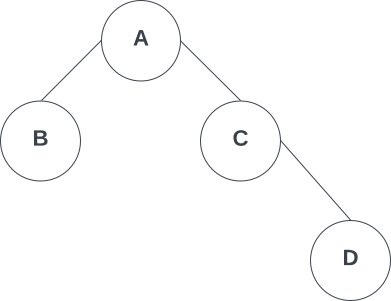
\includegraphics[
        width=6cm,
        keepaspectratio,
    ]{chapters/6. Eigenschaften binärer Bäume/img/ABCD}
    \caption{Ein \textit{transitiver Nachfolger} von $A$ ist $D$. Nur $B$ und $C$ sind \textit{direkte Nachfolger} von $A$. }
    \label{fig:ABCD}
\end{figure}

Mit \textit{Grad eines Knotens} (auch \textit{Rang}(vgl.~\cite[260]{OW17e})) wird die Anzahl seiner \underline{direkten Nachfolger} bezeichnet\footnote{siehe hierzu auch im Skript (Teil 2) Seite 101}.

\subsection*{Der Grad eines Blattes ist immer 0.}

Ein Knoten in einem Baum ist entweder ein \textit{innerer Knoten} oder ein \textit{Blatt}.
Ein \textit{innerer Knoten} ist ein Knoten, der mindestens einen Nachfolger besitzt.
Ein \textit{Blatt} ist ein Knoten, der keine Nachfolger hat, und deshalb den Grad $0$ besitzt\footnote{
auch in diesem Zusammenhang ist das Skript (Teil 2) auf Seite 101 sehr aussagekräftig.
}:

\blockquote[{\cite[259, Hervorhebungen i.O.]{OW17e}}]{
    Da die Menge der Knoten eines Baumes stets als endlich vorausgesetzt wird, muss es
    Knoten geben, die keine Söhne haben. Diese Knoten werden üblicherweise als \textit{Blätter}
    bezeichnet; alle anderen Knoten nennt man \textit{innere Knoten}.
}

\subsection*{Ein innerer Knoten ist ein Knoten mit einem Grad > 1.}
Mit den bis hierhin aufgeführten Kriterien {bzgl.} Grad eines Knotens darf man schließen, dass es richtigerweise ``mit einem Grad $>= 1$`` heißen muss\footnote{
    so auch im Skript (Teil 2) auf Seite 101 vermerkt.
}.


\subsection*{Ein Baum ist vollständig, falls alle inneren Knoten zwei direkte Nachfolger haben und alle Blätter die gleiche Tiefe aufweisen.}

Bestätigt u.a. durch \textit{Ottmann und Widmayer}:

\blockquote[{\cite[261, Hervorhebungen i.O.]{OW17e}}]{
    Ein Baum heißt vollständig, wenn er auf jedem \textit{Niveau} die maximal mögliche Knotenzahl hat und sämtliche Blätter dieselbe Tiefe haben.
}

Mit \textit{Niveau} werden bei \textit{Ottmann und Widmayer} Knoten gleicher Tiefe zusammengefasst.


\subsection*{Jedes Blatt eines Baumes hat dieselbe Höhe.}
Als \textit{Höhe} eines Baumes versteht man den maximalen Abstand eines Blattes von der Wurzel.

Der Abstand eines Knotens (und damit auch Blattes) von der Wurzel wird durch seine \textit{Tiefe} ausgedrückt\footnote{
dargestellt im Skript (Teil 2) auf Seite 102
}.

Damit jedes Blatt in einem Baum dieselbe Tiefe hat wie alle in dem Baum vorhandenen Blätter, muss der Baum \textit{vollständig sein}.
Richtigerweise müßte es also heißen: Jedes Blatt eines \underline{vollständigen Baumes} hat dieselbe Höhe.


